% A cubic graph with no perfect matching (generated by figs_c1ch06.py).
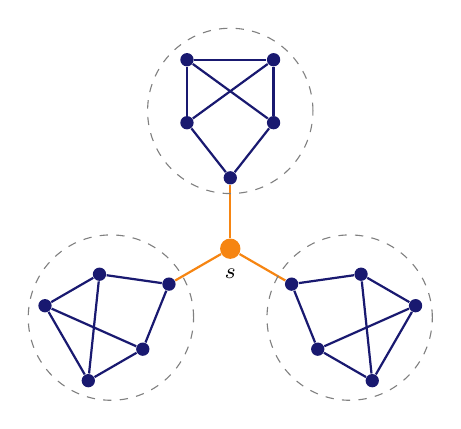
\begin{tikzpicture}[x=1cm,y=1cm,v/.style={circle,fill=MidnightBlue,inner sep=1.7pt},s/.style={circle,fill=BurntOrange,inner sep=2.6pt},e/.style={thick,MidnightBlue},b/.style={thick,BurntOrange}]
\node[s,label={[font=\footnotesize]below:$s$}] (s) at (0,0) {};
\node[v] (w0) at (0.000,0.900) {};
\node[v] (k10) at (-0.550,1.600) {};
\node[v] (k20) at (0.550,1.600) {};
\node[v] (k30) at (-0.550,2.400) {};
\node[v] (k40) at (0.550,2.400) {};
\draw[b] (s) -- (w0);
\draw[e] (w0) -- (k10);
\draw[e] (w0) -- (k20);
\draw[e] (k10) -- (k30);
\draw[e] (k10) -- (k40);
\draw[e] (k20) -- (k30);
\draw[e] (k20) -- (k40);
\draw[e] (k30) -- (k40);
\draw[gray,dashed] (0.000,1.750) circle (1.05);
\node[v] (w1) at (-0.779,-0.450) {};
\node[v] (k11) at (-1.111,-1.276) {};
\node[v] (k21) at (-1.661,-0.324) {};
\node[v] (k31) at (-1.803,-1.676) {};
\node[v] (k41) at (-2.353,-0.724) {};
\draw[b] (s) -- (w1);
\draw[e] (w1) -- (k11);
\draw[e] (w1) -- (k21);
\draw[e] (k11) -- (k31);
\draw[e] (k11) -- (k41);
\draw[e] (k21) -- (k31);
\draw[e] (k21) -- (k41);
\draw[e] (k31) -- (k41);
\draw[gray,dashed] (-1.516,-0.875) circle (1.05);
\node[v] (w2) at (0.779,-0.450) {};
\node[v] (k12) at (1.661,-0.324) {};
\node[v] (k22) at (1.111,-1.276) {};
\node[v] (k32) at (2.353,-0.724) {};
\node[v] (k42) at (1.803,-1.676) {};
\draw[b] (s) -- (w2);
\draw[e] (w2) -- (k12);
\draw[e] (w2) -- (k22);
\draw[e] (k12) -- (k32);
\draw[e] (k12) -- (k42);
\draw[e] (k22) -- (k32);
\draw[e] (k22) -- (k42);
\draw[e] (k32) -- (k42);
\draw[gray,dashed] (1.516,-0.875) circle (1.05);
\end{tikzpicture}
